\section{Chanllenges}

In this section, we articulate several chanllenges and existing problems
in quantifying the side-channel vulnerability leakages. We describe the
chanllenges and then briefly present the corresponding solution.

\subsection{Information Leakage Definition}
Existing static-based side-channel quantification works~\cite{182946} define information leakage
as the mutual information or the maximal leakage. Those definitions provide a strong security guarantee
when trying to prove a program is secure enough if the their methods calculate the program 
leaks zero bits of information.

However, the above definition is less useful to justify the sensitive level of leakage sites. 
Considering the example code~\ref{code::entropy} in the previous section, if an attacker knows the
code executes branch A by some observations, the attacker can know the key actually equals to 128. 
Suppose it is a dummy password checker, in which case the attacker can fully retrieve the password.
Therefore, the total information leakage should be 8 bits, which equals to the size
of unsigned char. 
According to the mutual definition, however, the leakage will be 1.7 bits. The maximal information
leakage is 2 bits. Both approaches fail to tell how much information is actually leaked
during the execution precisely.

The problem with the existing methods is that they are static-based and the 
input values are neglected by the previous definition. 
They assume the attacker runs the program multiple times with many different sensitive 
information as the input. Both the mutual information and the max-leakage give an ``average" 
estimate of the information leakage. But it isn't the typical scenario for an adversary to 
launch the side-channel attack. When a side-channel attack happens, the adversary wants 
to retrieve the sensitive information, in which case the sensitive information is fixed (e.g. AES keys). 
The adversary will run the attack over and over again and guess the value bit by bit. Like the 
previous example, the existing static method doesn’t work well in those situations.

\begin{figure}
\centering
\subfloat[Mutual Information]
{
    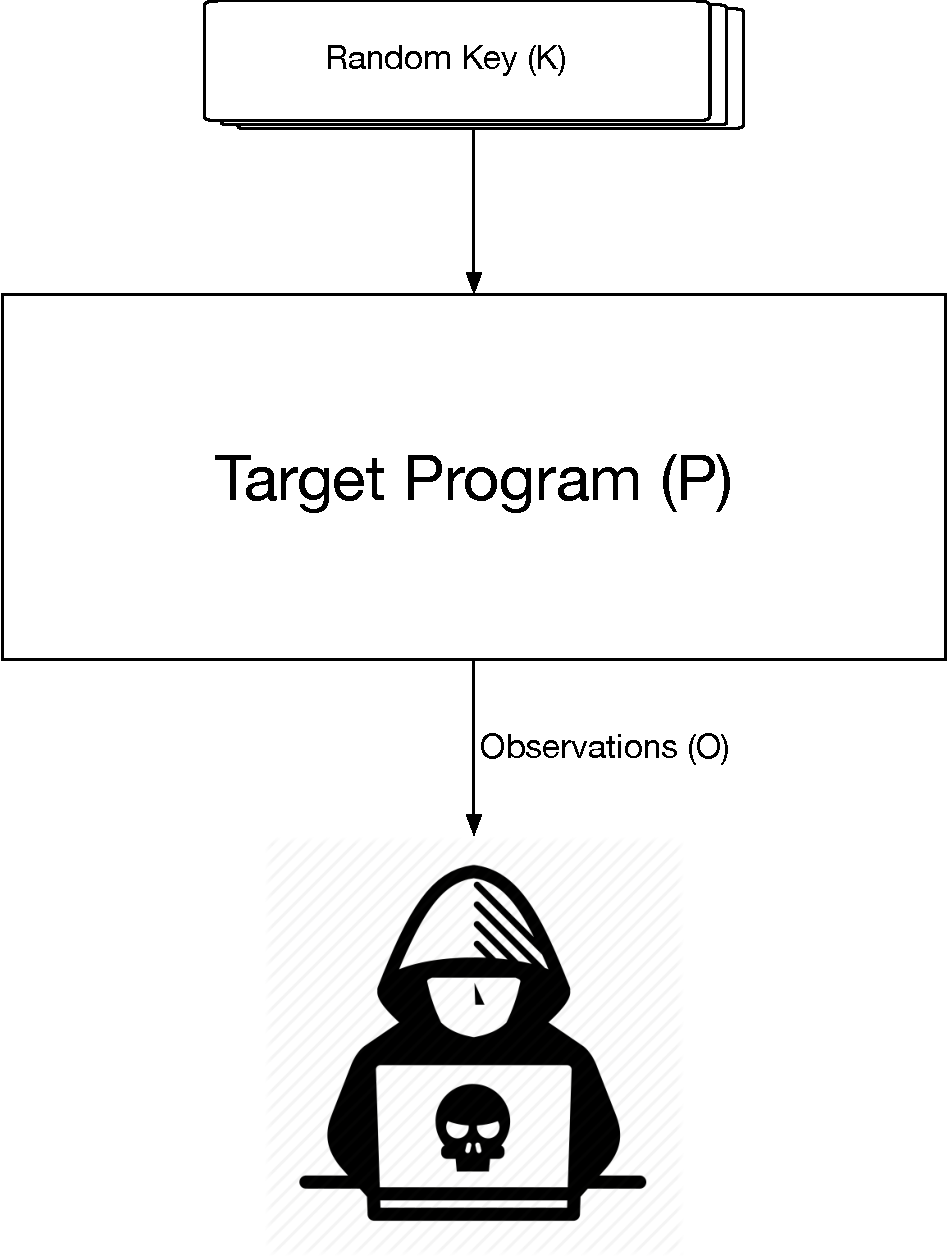
\includegraphics[width=.4\linewidth]{./figures/MI.pdf}
    \label{fig:1}
}
\subfloat[Real Attack]
{
    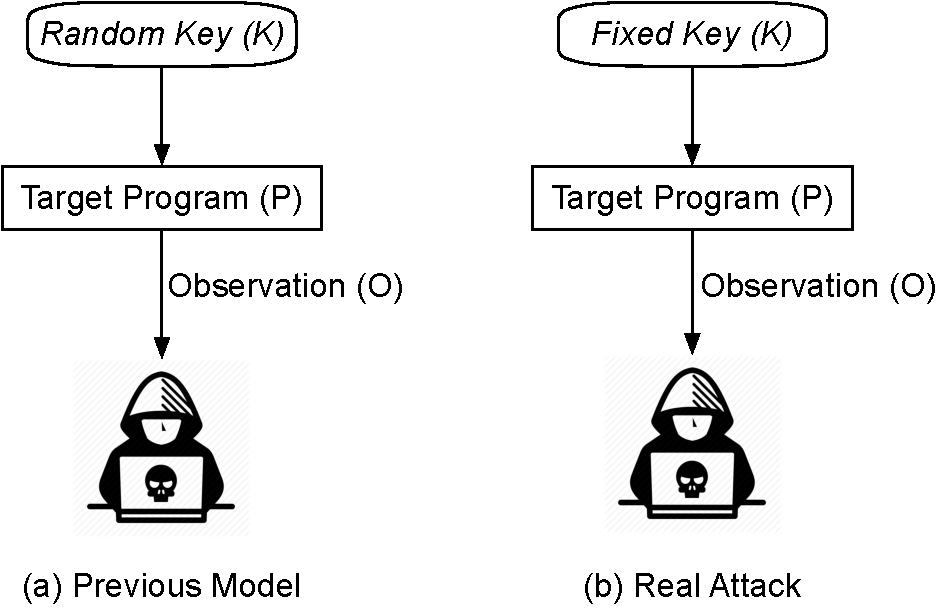
\includegraphics[width=.4\linewidth]{./figures/RA.pdf}
    \label{fig:2}
}
\end{figure}

\textbf{Solution:}
In the project, we hope to give a very precise definition of information leakages. 
Suppose an attacker run the target program mutiple times with one fixed input, we
want to know how much information he can infer by oberserving the memory access patterns.
We come to the simple slogan ~\cite{10.1007/978-3-642-00596-1_21} where the information
leakage equals:

\textbf{initial uncertainty - remaining uncertainty}

If an adversary has zero knowledge about the input before the attack. The initial uncertainty
equals to the size the input. As for the remaining uncertainty, we come to the original definition
of the information content.

We quantify the information leakage with the following definition. 

\newtheorem{mydef}{Definition}

\begin{mydef}
\label{def}
Given a program $P$ with the input set $K$, 
an adversary has the observation $o$ when the input $k{\in}K$. 
We denote it as
    $$P(k) = o$$
The leakage $L_{Pko}$ based on the oberservation is
    $$L_{Pko} = log_2{|K|} - log_2{|K^o|}$$
    where
    $$K^o = \{k^{'} | k^{'}{\in}K \ and \ P(k^{'}) = o \}$$
\end{mydef}

With the new definition, if the attacker observes that the code~\ref{code::entropy} runs the branch 1, 
then the $K^{o^{1}} = \{128\}$. Therefore, the information leakage $L_{Pko^{1}} = log_2{256} - log_2{1} = 8$
bits, which means the key is totally leaked. If the attacker observes the code runs other
branches, the leaked information is shown in the following table.

\begin{table}[h]
    \centering
    \resizebox{.7\columnwidth}{!}{
    \begin{tabular}{|c|c|c|c|c|}
    \hline
    Branch & 1 & 2  & 3  & 4   \\ \hline
    $K^o$   & 1 & 64 & 64 & 127 \\ \hline
    $L_{Pko}$(bits)   & 8 & 2  & 2  & 1   \\ \hline
    \end{tabular}
    }
    \caption{The leaked information by the definition~\ref{def}}
\end{table}

With the same definition~\ref{def}, if the attacker observes that the code run branch 2, the information
leakage will be 2 bits. The conclusion is consistent with the intuition. Because if the branch 2 was
executed, we can know the key is less than 64. So we know the most and the second significant digits of 
the value key equals to $128$.

\subsection{Multiple Leak Sites}
Real-world software can have various side-channel vulnerabilities. Those vulnerabilities 
may spread in the whole program. An adversary may exploit more than one side-channel vulnerabilities 
to gain more information~\cite{7163052, 191010}. For example, the controlled-side channel attack~\cite{7163052}, 
the author demonstrates an attack against a popular spell checking tool, Hunspell. By observing four sets 
of secret-dependent memory accesses sites in two functions $HashMgr::addword$ and $HashMgr::lookup$, 
the author can recover the word in the original text.

For the Hunspell, the attacker manually studies the source code of Hunspell, figure out
the relation of those vulnerabilities and launch the attack. In order to precisely quantify the
total information leakage, we need to know the relation of those leakage sites. 


\lstinputlisting[language=c, 
                 numbers=left,
                 numbersep=5pt,                   % how far the line-numbers are from the code
                 caption={Multiple leakages},
                 %frame = simple,
                 captionpos=b,
                 label={code::multiple},
                 basicstyle=\fontsize{7}{9}\selectfont\ttfamily]
                 {sample_code/motivation_multiple.c}

                

Considering the running example in ~\ref{code::multiple}, in which $k1$, $k2$ and $k3$ are
the sensitive key. The code has six different leakage. Leakage 1, 2, 3 are the secret-dependent
data accesses and leakage 4, 5, 6 are the secret-dependent control-flow transfers. It is
very hard to estimate total leakages. For example, the attacker can infer the last three digits of
$k1$, $k2$, $k3$ from leakage 1, 2, 3. So those leakages are independent. For leakage 1, 4, 6, however,
we have no idea about the total information leakage.

For the real program, it is tough to estimate the total information leakage for the following reasons.
First, the real-world applications have more than thousands of lines of code. Side-channel vulnerabilities
could exist in many different functions of the source code. One leakage site leaks the temporary value. 
But the value contains some information about the original buffer. It is hard to know how the 
the sensitive value affects the temporary value. Second, some leakages sites may be
dependent. The occurrence of the first affects the occurrence of the second sites. We 
can simply add them up. Third, leakage sites are in the different block of the 
control-flow graph, which means that only one of the two leakages site may execute
during the exectution.

Suppose one program has two side-channel vulnerabilities A and B, which leaks $L_A$ and $L_B$ bits
during the execution. The total leaked information is noted as $L_{Total}$. The relation between
A and B have the following three cases. 

\subsubsection{Independent Leakages}
If A and B are independent leakages, the total information leakage will be:
\begin{displaymath}
\label{independent leakage}
    L_{total} = L_A + L_B 
\end{displaymath} 

\subsubsection{Dependent Leakages}
If A and B are dependent leakages, the total information leakage will be:
\begin{displaymath}
\label{dependent leakage}
    \max{\{L_A, L_B\}}  <= L_{total} < L_A + L_B 
\end{displaymath}

\subsubsection{Mutual Exclusive Leakages}
If A and B are mutual exclusive leakges, then only A or B can be observed for one fixed input.
The total information leakage will be $L_A$ or $L_B$.

According to above definition, leakage 1, 2, 3 are independent leakages. Leakage 4, 5
are mutual exclusive leakages. 

\textbf{Solution: }We run the symbolic execution on the top of the execution traces.
At the beginning of the exectution,
each byte in the sensitive buffer is modeled with with a symbol. After that, the symbolic
exectution engine interprets each instruction of the exectution traces. So every values in the
registers or memory cells is modeled with a math formula.

Given a program $P$, $k$ is the sensitive input. The $k$ should be a value in a memory cell or a sequential 
buffer (e.g., an array). We use $k_i$ to denote the sensitive information, where $i$ is the index of the byte in
the original buffer. We can have the following equations. The t1, t2, t3, is the temporary values during the execution.

$$t_1 = f_1(k_1, k2, ... k_n)$$
$$t_2 = f_2(k1, k2, ... k_n)$$
$$t_3 = f_3(k1, k2, ... k_n)$$
$...$
$$t_m = f_m(k1, k2, ... k_n)$$

After that, we model each potential leakage sites as a math formulas.

The attacker can retrieve the sensitive information by observing the different patterns in 
control-flows and data access when the program process different sensitive information. 
We refer them as the secret-dependent control flow and secret-dependent data access accordingly.


\subsubsection{Secret-dependent Control Flow}
Here is an example of the secret-dependent control-flows. Consider the code snippet in List 1. 
Here the key is the confidential data. The code will have different behaviours (time, cache access) 
dependenting on which branch is actually executing. By observing the behaviour, 
the attacker can infer which branch actually executed and know some of the sensitive information. 
One of the famous leakage example is the square and multiply in many RSA implementations. 

For example, the attacker knows the key equals to zero if he observes the code run the branch1. 
Because key has 256 different possibilities. The original key has lg256 = 8 bits information. 
If the attacker can observe the code run branch 1. Then he will knows the key equals to zero. 
If the code run branch 2, the attacker can infer the key doesn’t equal to zero. 

\begin{lstlisting}
Branch 1
temp = 0xb;
0 =< key <= 256;
temp = key/2;
\end{lstlisting}

Information Leakage = -log(1/p) = -log(1/256) = 8 bits

\begin{lstlisting}
Branch 2
temp != 0; 
0 =< key <= 256;
temp = key/2;
\end{lstlisting}

Information Leakage = -log(255/256) bits

\subsubsection{Seret-dependent Memory Access}

\begin{lstlisting}

T[64]; // Lookup tables with 64 entries
index = key % 63;
temp = T[index]; 
// Secret-dependent memory access       

\end{lstlisting}

The simple program above is an example of secret dependent memory access. 
Here T is a precomputed tables with sixty-four entries. 
Depending on the values of key, the program may access any values in the array. 
Those kind of code patterns may wildly exist in many crypto and media libraries. 

Suppose the attackers observe the code accesses the first entry of the lookup tables. 
We can have the following formulas.

\begin{lstlisting}
key mod 63 = 1
0 =< key <= 256
\end{lstlisting}

So the key can be one of the following values:
1 64 127 190 253

Information leakages = -log(5/256) =  5.6 bits


\subsection{Scalability and Performance}

After we transfer each potential leaks sites into logic formula. We can group several formulas together
to estimate the total information leakage. One naive way is to use the Monte Carlo sampling  estimate the
number of input keys. With the definition ~\ref{def}, we can estimate the total information leakage.

However, some pre-experiments show that above approach suffers from the unberable cost, which impede its usage
to detect and quantify side-channel leakages in real-world applications. 
We systematically analyze the performance bottlenecks of the whole process. In general, the performance suffers
from the two following reasons. 
\begin{itemize}
    \item Symbolic Execution. 
    \item The Naive Monte Carlo Sampling.
\end{itemize}
\subsubsection{Symbolic Execution}
Symbolic execution interprets each instruction and update the memory cells and registers with a 
formula that captured the sementics of the exectution. Unfortunately, the number of machine instructions 
are huge and the sementics of each instruction is complex. For example, the Intel Developer Manual~\cite{intelsys}
introduces more than 1000 different X86 instructions. It is tedious to manually implement the
rules for every instructions.

Therefore, existing binary analysis tools ~\cite{shoshitaishvili2016state, 10.1007/978-3-642-22110-1_37} 
will translate machine instructions into intermediate languages (IR). The IR typically has fewer 
instructions compared to the original machine instructions. The IR layer designs, which significantly
simplify the implementations, also introduce significant overhead as well~\cite{217563}.

\textbf{Solution: }We adopt the similar approach from~\cite{217563} and implement the symbolic exectution 
directly on the top X86 instructions.

\subsubsection{Monte Carlo Sampling}
For an application with $m$ bytes secret, there are total $2^{8m}$ possible inputs. Of the
$2^{8m}$ possible secrets, we want to know many of them of satisfy the given logic formula groups.
Then we can use the definition ~/ref{def} to calculate the information leakage.

A Monte Carlo method for approximating the number of satisfied values $|K_o|$ is to pick up 
$M$ random values and check how many of those numbers satisfy those constrains. If $l$ values
satisfy those constrains, then the approximating result is $\frac{l*2^{8m}}{M}$.

However, the number of satisfying values could be exponentially small. Considering the formula
$F={k_1} = 1\land{k_2} = 2\land{k_3} = 3\land{k_4} = 4$, $k_1$, $k_2$, $k_3$ and $k_4$ each represent
one byte in the sensitive buffer, there is only one possible solution of $2^{32}$ possible
values. The naive Monte Carlo Method also suffers from the curse of dimensionality. For example, 
the libjpeg libraries can transfer the image from one format into another format. One image could
be 1kMB. If we take each byte in the original buffer as symbols, the formula can have at most
1024 symbols. 

\textbf{Solution: }We adopt the Markov Chain Monte Carlo to estimate the number of possible input
that satisfies the logic formula groups. The key idea is that we have one group of input that satisfies
the logic formula constrains. We can also estimate the error with chebyshev inequality. We will
introduce the method in the following sections.
